\documentclass[a4paper,10pt]{article}
\usepackage[utf8]{inputenc}
\usepackage{geometry}
\geometry{margin=1in}
\usepackage{amsmath}
\usepackage{graphicx}
\usepackage{listings}
\usepackage{xcolor}
\usepackage{caption}
\usepackage{booktabs}
\usepackage{hyperref}

\lstset{
    language=R,
    basicstyle=\ttfamily\small,
    keywordstyle=\color{blue},
    commentstyle=\color{green!50!black},
    stringstyle=\color{red},
    numbers=left,
    numberstyle=\tiny,
    stepnumber=1,
    numbersep=5pt,
    showspaces=false,
    showstringspaces=false,
    frame=single,
    breaklines=true,
    breakatwhitespace=true,
    tabsize=2
}

\title{STAT0011 Decision and Risk In-Course Assessment 2025 \\ Group 5}
\author{}

\begin{document}

\maketitle

\section{Individual contributions}
\textbf{22002200}
\begin{itemize}
    \item Did this
    \item Done that
\end{itemize}
\textbf{22002200}
\begin{itemize}
    \item Did this
    \item Done that
\end{itemize}


\section{Introduction}
This report presents the analysis conducted by Group 5 for the STAT0011 Decision and Risk In-Course Assessment 2025. We evaluate the market risk of an equally-weighted portfolio comprising two stock indices, the S\&P 500 and the Shanghai Stock Exchange (SSE) Composite Index, using...

\section{Data Description}
We selected the S\&P 500 and SSE Composite Index from the six candidate indices provided. Weekly closing prices were obtained from \href{https://finance.yahoo.com}{Yahoo Finance} for the period spanning January 2000 to December 2023, yielding 1214 observations per index. Log-returns were calculated as follows:
\[
\text{ret}_t = \ln\left(\frac{P_t}{P_{t-1}}\right),
\]
where $P_t$ denotes the price at week $t$. The datasets are stored in \texttt{SP500.csv} and \texttt{SSE.csv}.

\section{Methodology}
\subsection{Modelling of log returns}
Something...

\subsection{Jarque-Bera tests}
Something...

\subsection{PIT}
Something...

\subsection{Estimation and Model Checking}
Something...

\subsection{Kolmogorov-Smirnov test}
Something...

\subsection{Anderson-Darling test}
Something...

\subsection{Error independence}
Something...

\subsection{Copula Modelling}
Something...

\subsection{Value-at-Risk using Monte Carlo simulation}
We simulated 100,000 scenarios...

\subsection{Beautiful table for something}
\begin{table}[h]
    \centering
    \caption{Table caption}
    \label{tab:dist}
    \begin{tabular}{lcc}
        \toprule
        Conditional Distribution & AIC & BIC \\
        \midrule
        Normal (norm) & -1.934944 & -4.901724 \\
        Student-t (std) & -4.977397 & -4.939430 \\
        Skew Student-t (sstd) & -5.009752 & -4.967040 \\
        Skew Normal (snorm) & -4.988160 & -4.950193 \\
        Skew Generalized Error (sged) & -5.005165 & -4.962453 \\
        Generalized Error (ged) & -4.970248 & -4.932282 \\
        \bottomrule
    \end{tabular}
\end{table}

\section{R Code}
Below is the R code used for the analysis:

\begin{lstlisting}
# Code to be inserted here
\end{lstlisting}

\section{Results}
Results to be inserted here

\section{Conclusion}
Using copula-based Monte Carlo simulation, we estimated the 95\% and 99\% 1-week VaR for an equally-weighted portfolio of S\&P 500 and SSE Composite Index. These values reflect...

\section{Figures}
\begin{figure}[h]
    \centering
    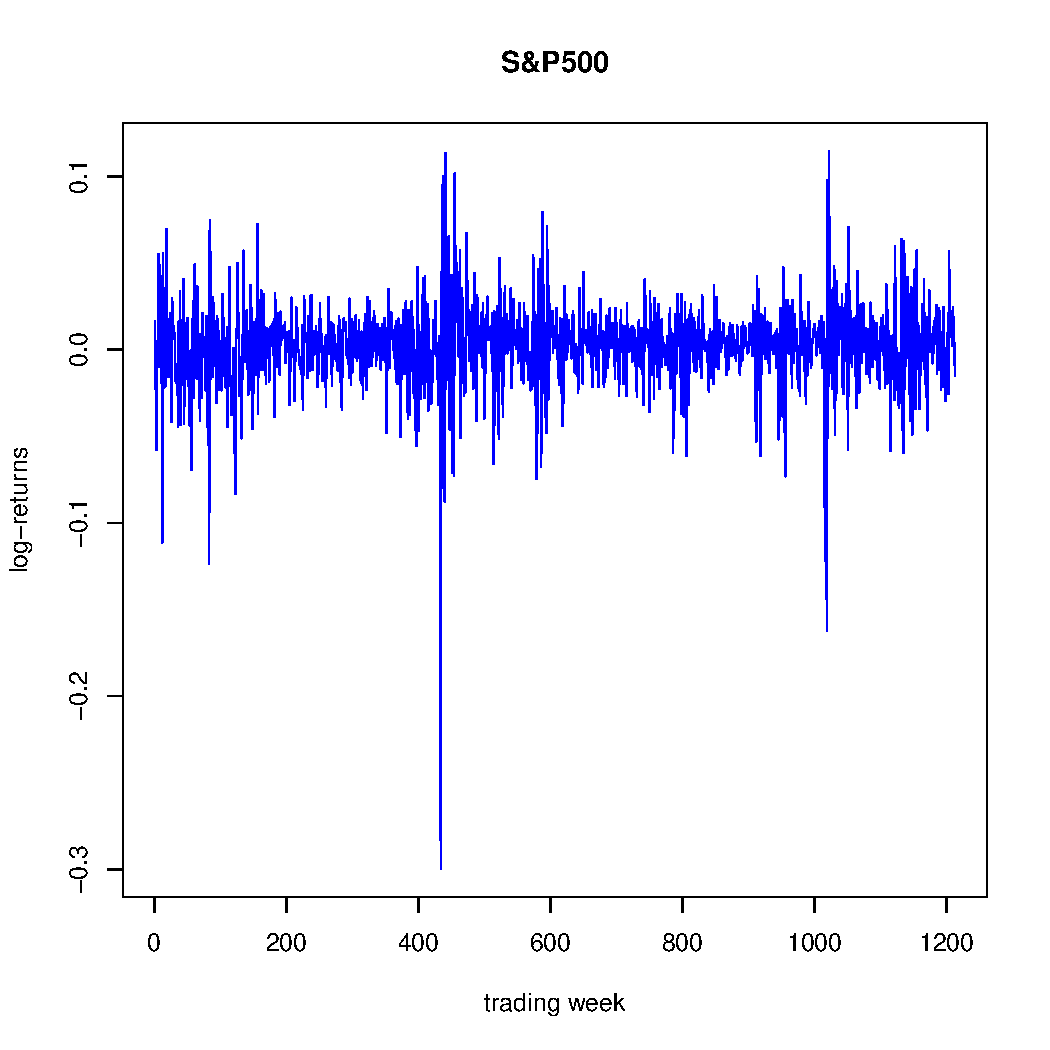
\includegraphics[width=0.9\textwidth, page=1]{Rplots.pdf}
    \caption{First plot from R analysis of the S\&P 500 and SSE Composite Index log-returns.}
    \label{fig:rplots1}
\end{figure}

\begin{figure}[h]
    \centering
    \includegraphics[width=0.9\textwidth, page=2]{Rplots.pdf}
    \caption{Second plot from R analysis.}
    \label{fig:rplots2}
\end{figure}

\begin{figure}[h]
    \centering
    \includegraphics[width=0.9\textwidth, page=3]{Rplots.pdf}
    \caption{Third plot from R analysis.}
    \label{fig:rplots3}
\end{figure}


\end{document}
